\section*{Materiali e Metodi}

\subsection*{Strumentazione}

L'esperimento è stato effettuato utilizzando il Mobile Universal Surface Explorer, detto MOUSE, che consiste in una scatola cubica di lato $12\,cm$ contenenete un magnete permanente a ferro di cavallo e una bobina piatta, su cui è posto il campione da studiare. 
La geometria piatta della bobina consente di trasmettere l'impulso a distanza dalla bobina stessa. 

Il MOUSE è stato realizzato per generare un campo magnetico con gradiente costante lungo l'asse $y$ per la componenente $B_z$, dove gli assi sono riferiti in figura \ref{fig:Str.png}. 

\begin{figure}[h!]
\centering
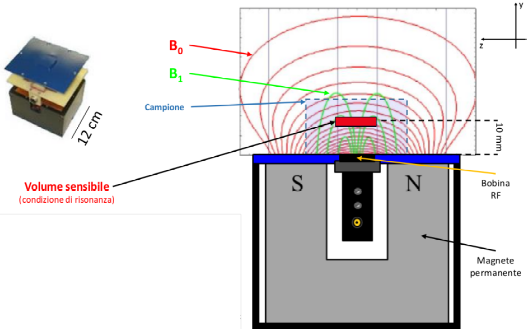
\includegraphics[scale=0.3]{Figure/Str.png}
\caption{Strumentazione.}
\label{fig:Str.png}
\end{figure}

Nonostante tale scopo, solo in una certa regione dello spazio è garantita con buona affidabilità un gradiente che sia costante e tale regione è denominata volume sensibile.
Lo spessore del volume sensibile è dipendente dalla larghezza della banda di frequenze che si stimolano.

In questa esperienza il volume sensibile è individuato a un'altezza di $3\,mm$ dalla base di appoggio del MOUSE e il valore del gradiente presente in questa regione è pari a $17\, \frac{T}{m}$.
Lo spessore di questo volume è tra $250-300\, \mu m$ essendo che l'impulso è stato inviato a $13.88\,MHz$ per una durata di $4.5\,ms$. 

I campioni studiati in questo esperimento sono l'acqua, il soltrol 130 e il soltrol 170.
Questi ultimi due sono idrocarburi paraffinici che si presentano come liquidi oleosi e sono sostanze utilizzate come solventi in vari campi di ricerca.

In realtà, il campione di acqua è una soluzione acquosa contentente una piccola percentuale di sale EDTA e rame.
Il rame legandosi con l'EDTA tende ad accorciare il tempo di rilassamento dell'acqua ma, data la piccola percentuale occupata, ha come unico effetto l'aumento del rapporto segnale rumore.

\'E importante sottolineare infatti che a differenza delle bobine solenoidali, le bobine piatte hanno un rapporto segnale rumore di circa due ordini di grandezza inferiore, visto che trasmettono a distanza.

\subsubsection*{CPMG}
Il metodo \textit{Carr-Purcell-Meiboom-Gill} viene usato per ottenere una misura di $T_2$ priva dei bias causati dalla non uniformità del campo magnetico applicato $B_0$ e dagli effetti di diffusione molecolare interni al campione.

Queste imperfezioni, infatti, fanno sì che con una misura tramite FID venga sempre misurato un tempo di rilassamento $T_2^*$ molto minore del $T_2$ "vero", causato solo dalle interazioni intrinseche del sistema. Inoltre, il metodo CPMG risulta più efficace rispetto al metodo Spin Echo (SE) in quanto riduce consistentemente gli effetti di diffusione molecolare, causati sempre dal gradiente del campo magnetico $B_0$.

Il metodo CPMG può essere presentato come un ampliamento del metodo SE: ottenuto un segnale di NMR con un segnale di impulso di $90^\circ$, si vogliono rimuovere gli effetti di decadimento causati dalla inomogeneità di $B_0$ applicando segnali di inversione di $180^\circ$. Tuttavia, invece di applicare un solo segnale di inversione a diversi tempi $\tau_i$ per poi misurare le conseguenti ampiezze di segnale di eco di spin, si va ad applicare una sequenza di segnali di inversione $(\tau_0 - 180^\circ - \tau_0)_n$ dove $\tau_0$ è il tempo più breve possibile ottenibile a livello strumentale.\\

Riassumendo, con un metodo di acquisizione tramite FID si misura un tempo di decadimento $T_2^*$, che in letteratura viene spesso assunto nella forma:
\begin{equation}
	\frac{1}{T_2^*} = \frac{1}{T_2} +\frac{1}{T_2'}
\end{equation}
dove $T_2'$ è la componente di tempo causata dalle imperfezioni del campo $B_0$.

Con il metodo SE, si riesce ad isolare meglio $T_2$. Tuttavia, rimangono gli effetti di diffusione molecolare che inevitabilmente interferiscono ancora con la misura. Indicando con $\tau$ il tempo di attesa prima del segnale di inversione, con $A(2\tau)$ l'ampiezza dell'eco al tempo $2\tau$ e con $A(0)$ il primo segnale NMR rilevato, si ha che:
\begin{equation}
	A(2\tau) = A(0)\exp\left(-\left(\frac{2\tau}{T_2}\right) - \frac{2}{3} \gamma^2 g^2 D \tau^3\right)
\end{equation}
dove $\gamma$ è ..., $g$ è ... e $D$ è ...

Con il metodo CPMG, invece, si riescono a confinare gli effetti di diffusione. essendo $\tau_0$ costante ed avendo molteplici segnali di eco di spin, si ha che:
\begin{equation}
	A(t) = A(0)\exp\left(-\left(\frac{t}{T_2}\right) - \frac{1}{3} \gamma^2 g^2 D \tau^2\right)
\end{equation}

Per visualizzare meglio il processo CPMG, si rimanda il lettore alla Figura \ref{fig:cpmg}.

\begin{figure}
\centering
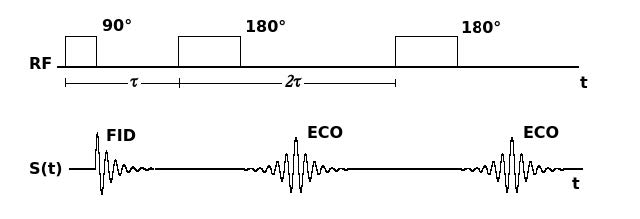
\includegraphics[width=\textwidth]{Figure/cpmg.jpg}
\caption{Segnale ottenuto tramite sequenza di impulsi CPMG.}
\label{fig:cpmg}
\end{figure}


\subsection*{Analisi dati tramite software UPENWin}

Il segnale acquisito è una curva multi-esponenziale nella forma:
\begin{equation}
	S(t) = \sum_{k=0}^M a_k \exp(-t/T_{1/2_k})
\end{equation}
dove si indica con $k$ una delle tante componenti del materiale non uniforme che presenta inevitabilmente tempi di rilassamento $T_1$ e $T_2$ differenti.

Tramite algoritmo UPEN (\textit{Uniform PENality}), implementato nel software UPENWin, si reinterpreta il segnale come una distribuzione continua dei tempi di rilassamento in forma integrale:
\begin{equation}
	S(t) = \int f(T_{1/2}) \exp(-t/T{1/2}) \, dT_{1/2}
\end{equation}
dove $f(T_{1/2})$ è una funzione di distribuzione dei tempi di rilassamento. Per invertire quindi il segnale acquisito ed ottenere una espressione valida della funzione di distribuzione, essendo possibili infinite soluzioni a causa degli errori sperimentali associati ad ogni dato acquisito, il software UPEN fornisce una stima di soluzione in base ad un principio di penalizzazione di soluzioni con eccessivi picchi distinti e non sufficientemente giustificati dai dati.

\subsection*{Analisi}

Il coefficiente di diffusione è stato ricavato ripetendo più volte la sequenza CPMG su ciascun campione aumentando progressivamente il tempo di echo($T_E$) e quindi $\tau$, pari alla metà di $T_E$.
Come spiegato nella sezione introduttiva, in questo modo è possibile  valutare quanto la diffusione influenzi il tempo di rilassamento.

Grazie al software Upen è stato possibile elaborare i dati in modo da poter rappresentare il rilassamento sia ponendo in relazione il tempo di acquisizione con l'intensità di segnale, che la scala dei tempi di rilassamento con la densità del segnale.

La prima fase di analisi ha previsto l'analisi qualitativa tra le immagini ottenute aumentando $\tau$ in modo da trarre le prime informazioni riguardo al rilassamento.
L'effetto atteso da queste analisi qualitative è in primo luogo il progressivo aumento dell'inclinazione delle rette descritte nel grafico semilogaritmico del tempo di acquisizione e dell'intensità di segnale.
In aggiunta è attesa la progressiva traslazione dei picchi delle curve presenti nel grafico tra i tempi di rilassamento e la densità del segnale.

In seguito sono state calcolate le stime dei tempi di rilassamento $T_2$ dei vari picchi per verificare la relazione espressa dall'equazione \ref{eq:R}. 
\'E stato quindi tracciato un grafico che descrivesse la relazione \ref{eq:R}, considerando come variabile indipendente $\tau^2$($x$). 

In particolare è stata eseguita una regressione lineare pesata per ottenere il coefficiente angolare dell'equazione.
Da questo è stato calcolato il coefficiente di autodiffusione analiticamente considerando che $D=\frac{3A}{{\gamma}^2}g^2$.

Per quanto riguarda le incertezze associate alle grandezze, è stato considerato come errore sul coefficiente angolare l'incertezza proviente dal best fit pesato; mentre per il coefficiente di autodiffusione è stata semplicemente propagata l'incertezza relativa di tale grandezza.


